% !TeX root = ../../main.tex
\newpage
\section{Generator sztucznych danych}
\label{sec:generator}

Problem skompletowania dostatecznie licznego zbioru treningowego (wspomniany w Rozdziale \numberref(sec:wyzwania)) został rozwiązany poprzez stworzenie generatora sztucznych obrazów.
Generator, zaimplementowany jako scena 3D w JavaScript pozwala na generowanie obrazów z~następującymi cechami:

\begin{itemize}
	\item zmienne kolory obiektów na obrazie, to jest podłogi, kortu, słupków;
	\item zmieniające swoją pozycję źródła światła, a co za tym idzie zmienny kierynek i rozmiar rzucanych cieni;
	\item zmienna pozycja zawodników na korcie, 
	\item zmienne odległości między kortami, odzwierciedlające różnice między placówkami w których odbywają się zawody sportowe.
\end{itemize}

Dzięki powyższym cechom możliwe jest przygotowanie sztucznych obrazów zbliżonych do obrazów z kamer przemysłowych stosowanych na meczach odbywających się w różnych lokalizacjach.

W celu, aby obraz stanowił rekord treningowy, wymagana jest tak zwana anotacja, czyli oznaczenie obszaru kortu. Rysunek \myfigrefx{fig:annotated_fake} przedstawia przykład anotacji na sztucznie wygenerowanym obrazie obrazie.
Zbiór danych treningowych złożony z wygenerowanych sztucznych danych zawiera 72 obrazy o rozdzielczości 800x600 pikseli.

\begin{figure}[!htb]
  \minipage{0.45\textwidth}
    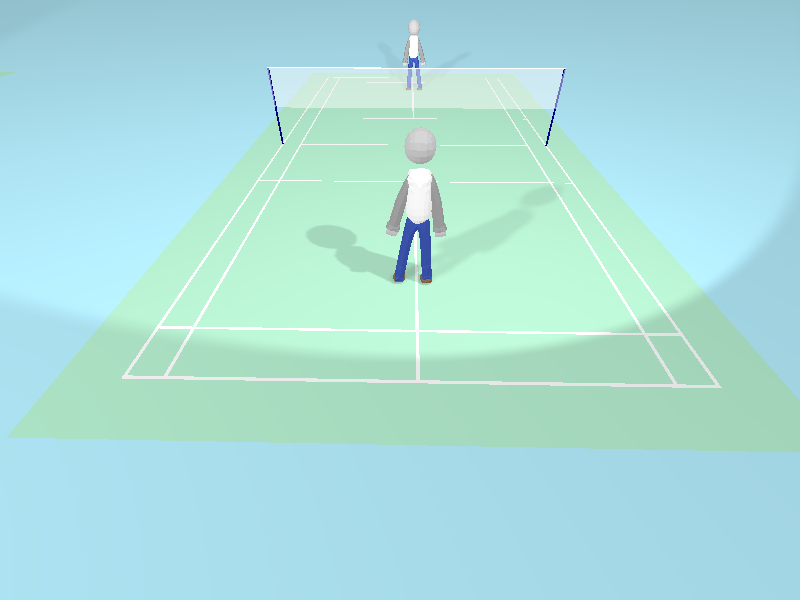
\includegraphics[width=\linewidth]{./fake.jpg}
    \caption{Przykład wygenerowanego sztucznego obrazu.}
  \endminipage\hfill
  \minipage{0.45\textwidth}
    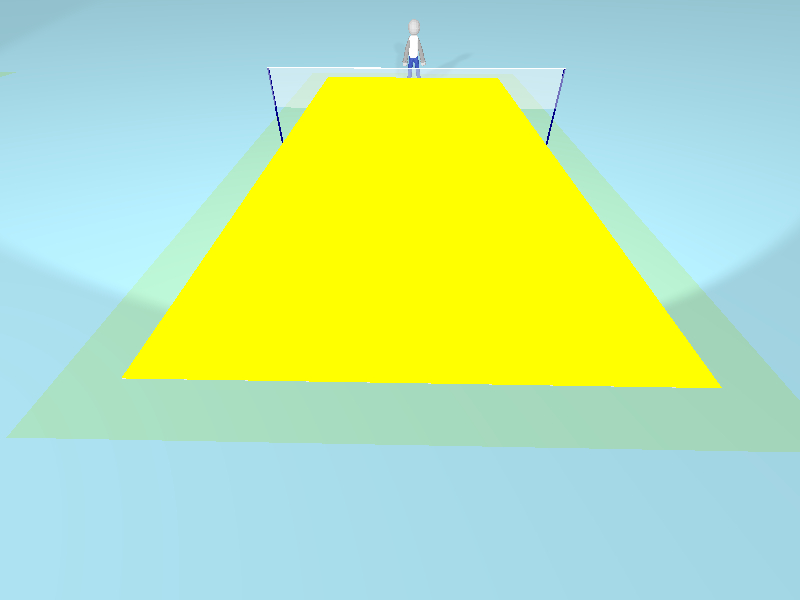
\includegraphics[width=\linewidth]{./fake_annotated.jpg}
    \caption{Przykład wygenerowanego sztucznego obrazu z zaznaczoną anotacją powierzchni kortu.}
    \label{fig:annotated_fake}
  \endminipage\hfill
\end{figure}
